\newpage

\section{Actividad 4: DIAC}

\subsection{Actividad de Laboratorio}

\begin{itemize}
    \item DIAC DB3.
    \item Dos multímetros.
    \item Resistores varios.
    \item Fuente de alimentación de 0 a 600V.
\end{itemize}

\paragraph{Procedimiento}
Se montó el siguiente circuito:\\
\includegraphics[width=8cm]{./imagenes/Circ4.png}

Variamos la tensión de alimentación de 0 a 50V, midiendo la corriente y caída de tensión en el DIAC.\\
Luego invertimos los terminales del DIAC y repetimos el procedimiento anterior.\\

Como resultados obtenemos las siguientes tablas y el siguiente gráfico:


\begin{table}[ht]
\centering
\begin{tabular}{|>{\columncolor[HTML]{FFCCC9}}c |c|c|}
\hline
\cellcolor[HTML]{FFFC9E}$V_{CC}${[}V{]} & \cellcolor[HTML]{FFFC9E}$V_{AK}${[}V{]} & \cellcolor[HTML]{FFFC9E}$I_A${[}mA{]} \\ \hline
0    & 0    & 0    \\ \hline
5    & 5    & 0    \\ \hline
10   & 10   & 0    \\ \hline
15   & 15   & 0    \\ \hline
20   & 20   & 0    \\ \hline
22   & 22   & 0    \\ \hline
25   & 25   & 0    \\ \hline
28   & 28   & 0    \\ \hline
30   & 30   & 0    \\ \hline
32   & 23.8 & 1.74 \\ \hline
34.3 & 23.4 & 2.24 \\ \hline
40.4 & 22.6 & 3.72 \\ \hline
45   & 22.2 & 4.9  \\ \hline
50   & 21.9 & 5.92 \\ \hline
\end{tabular}
\caption{Mediciones de $I_A$ frente a $V_{AK}$.}
\end{table}

\begin{table}[ht]
\centering
\begin{tabular}{|>{\columncolor[HTML]{FFCCC9}}c |c|c|}
\hline
\cellcolor[HTML]{FFFC9E}$V_{CC}${[}V{]} & \cellcolor[HTML]{FFFC9E}$V_{AK}${[}V{]} & \cellcolor[HTML]{FFFC9E}$I_A${[}mA{]} \\ \hline
0    & 0    & 0    \\ \hline
5    & -5    & 0    \\ \hline
10   & -10   & 0    \\ \hline
15   & -15   & 0    \\ \hline
20   & -20   & 0    \\ \hline
22   & -22   & 0    \\ \hline
25   & -25   & 0    \\ \hline
28   & -28   & 0    \\ \hline
30   & -30   & 0    \\ \hline
32   & -23.7 & -1.72 \\ \hline
34.3 & -23.4 & -2.26 \\ \hline
40.4 & -22.6 & -3.7 \\ \hline
45   & -22.2 & -4.8  \\ \hline
50   & -21.9 & -5.9 \\ \hline
\end{tabular}
\caption{Mediciones de $I_A$ frente a $V_{AK}$.}
\end{table}


\begin{figure}[ht]
\centering
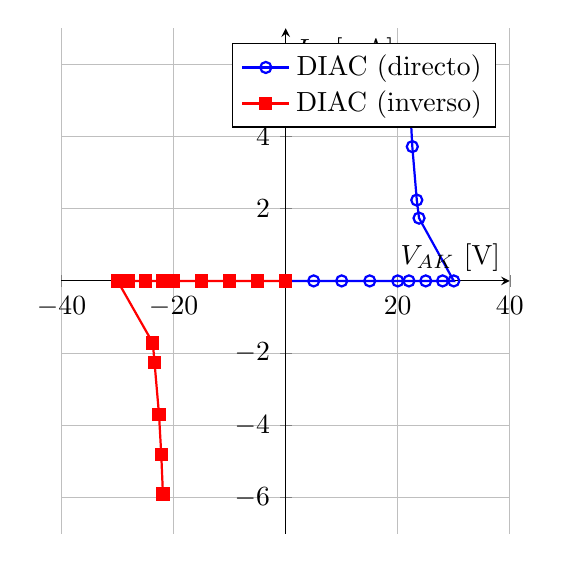
\begin{tikzpicture}
\begin{axis}[
    width=0.6\textwidth,
    height=8cm,
    xlabel={$V_{AK}$ [V]},
    ylabel={$I_A$ [mA]},
    xmin=-40, xmax=40,
    ymin=-7, ymax=7,
    grid=both,
    legend pos=north east,
    axis x line=middle,
    axis y line=middle,
    cycle list name=color list
]
% Direct orientation
\addplot+[mark=o, thick, blue] coordinates {
    (0,0) (5,0) (10,0) (15,0) (20,0) (22,0) (25,0) (28,0) (30,0) (23.8,1.74) (23.4,2.24) (22.6,3.72) (22.2,4.9) (21.9,5.92)
};
\addlegendentry{DIAC (directo)}

% Inverse orientation
\addplot+[mark=square*, thick, red] coordinates {
    (0,0) (-5,0) (-10,0) (-15,0) (-20,0) (-22,0) (-25,0) (-28,0) (-30,0) (-23.7,-1.72) (-23.4,-2.26) (-22.6,-3.7) (-22.2,-4.8) (-21.9,-5.9)
};
\addlegendentry{DIAC (inverso)}
\end{axis}
\end{tikzpicture}
\caption{Curva experimental $I_A$ frente a $V_{AK}$ para ambas polaridades.}
\end{figure}



\paragraph{Análisis de Resultados}

Como podemos observar en la figura de arriba, en el DIAC el voltaje Vak se eleva lentamente hasta llegar a un punto de ruptura, donde la corriente aumenta rápidamente y el voltaje cae abruptamente. Este comportamiento es similar al de un SCR visto anteriormente, pero en este caso, tambien es posible hacerlo en la dirección inversa, ya que el DIAC es un dispositivo simétrico, tal y como vemos en la segunda parte en donde se obtuvo la grafica para la polaridad inversa.\\